% !TEX program = xelatex
\documentclass[aspectratio=169]{beamer}
\usepackage{amsmath}
\usepackage{amssymb}
\usepackage{graphicx}
\usepackage{tcolorbox}
\usepackage{booktabs}
\usepackage{colortbl}
\usepackage{xcolor}
\usepackage{tikz}
\usetikzlibrary{angles,quotes}
\usepackage[utf8]{inputenc}

% Custom colors
\definecolor{primary}{RGB}{41, 128, 185}
\definecolor{secondary}{RGB}{52, 152, 219}
\definecolor{accent}{RGB}{231, 76, 60}
\definecolor{lightgray}{RGB}{236, 240, 241}

% Theme customization
\usetheme{Madrid}
\usecolortheme{whale}
\setbeamercolor{structure}{fg=primary}
\setbeamercolor{background canvas}{bg=white}
\setbeamercolor{normal text}{fg=black}

% Title page info
\title{Pre-Calculus 11}
\subtitle{Chapter 8.2: Quadratic Inequalities with One Variable}
\author{Created by Yi-Chen Lin}
\date{\today}

\begin{document}

% Title Page
\begin{frame}
    \titlepage
\end{frame}

% What is a Quadratic Inequality?
\begin{frame}{What is a Quadratic Inequality?}
    \begin{tcolorbox}[colback=lightgray,colframe=primary,title=Definition]
        \footnotesize
        A quadratic inequality is an inequality that can be written in the form:
        \begin{itemize}
            \item $ax^2 + bx + c > 0$
            \item $ax^2 + bx + c \geq 0$
            \item $ax^2 + bx + c < 0$
            \item $ax^2 + bx + c \leq 0$
        \end{itemize}
        where $a$, $b$, and $c$ are real numbers and $a \neq 0$
    \end{tcolorbox}
    \vspace{0.5em}
    \textbf{Examples:}
    \begin{itemize}
        \item $x^2 > 16$
        \item $x^2 - 5x - 14 \leq 0$
    \end{itemize}
\end{frame}

% Steps to Solve Square Inequalities
\begin{frame}{How to Solve Square Inequalities}
    \begin{tcolorbox}[colback=lightgray,colframe=primary,title=Step-by-Step Method]
        \footnotesize
        \begin{enumerate}
            \item \textcolor{accent}{\textbf{Isolate the square term:}}
            \begin{itemize}
                \item Move all terms to one side
                \item Square root both sides
            \end{itemize}
            \item \textcolor{accent}{\textbf{Consider both positive and negative roots}}
            \item \textcolor{accent}{\textbf{Draw a number line}} and mark the roots
            \item Test points in each domain
            \item \textcolor{accent}{\textbf{Write the solution}} using interval notation
        \end{enumerate}
    \end{tcolorbox}
\end{frame}

% Example: Solve x² > 16
\begin{frame}{Example: Solve $x^2 > 16$}
    \begin{columns}
        \column{0.5\textwidth}
        \begin{tcolorbox}[colback=secondary!10,colframe=primary,title=Solution]
            \footnotesize
            \begin{align*}
                x^2 &> 16 \\
                x &< -4 \text{ or } x > 4
            \end{align*}
            Test points:
            \begin{itemize}
                \item $(-5)^2 = 25 > 16$ [True]
                \item $(0)^2 = 0 < 16$ [False]
                \item $(5)^2 = 25 > 16$ [True]
            \end{itemize}
        \end{tcolorbox}
        
        \column{0.5\textwidth}
        \begin{center}
        \begin{tikzpicture}[scale=0.7]
            \draw[->] (-6,0) -- (6,0);
            \foreach \x in {-4,0,4}
                \draw (\x,0.2) -- (\x,-0.2) node[below] {\x};
            \draw[orange,thick,->] (-6,0) -- (-4,0);
            \draw[orange,thick,->] (4,0) -- (6,0);
        \end{tikzpicture}
        \end{center}
    \end{columns}
\end{frame}

% Steps for Quadratic Inequalities
\begin{frame}{Solving Quadratic Inequalities by Factoring}
    \begin{tcolorbox}[colback=lightgray,colframe=primary,title=Method]
        \footnotesize
        \begin{enumerate}
            \item \textcolor{accent}{\textbf{Factor}} the quadratic expression
            \item Find the \textcolor{accent}{\textbf{roots}} [solutions]
            \item Draw a \textcolor{accent}{\textbf{parabola}} and mark the roots
            \item Determine if points satisfy the inequality:
            \begin{itemize}
                \item Above/Below/Equal to the X-axis
            \end{itemize}
            \item The domain that satisfies the inequality is the solution
        \end{enumerate}
    \end{tcolorbox}
\end{frame}

% Example: Solve x² - 5x - 14 ≤ 0
\begin{frame}
    % Blue header bar
    \begin{beamercolorbox}[wd=\paperwidth,ht=1.5cm,dp=0.2cm]{structure}
        \hspace{0.5cm}\Large Example: Solve $x^2 - 5x - 14 \leq 0$
    \end{beamercolorbox}
    
    \vspace{0.3cm}
    \begin{columns}[T]
        \column{0.4\textwidth}
        % Simple blue border box for solution
        \begin{tcolorbox}[
            colback=white,
            colframe=primary,
            arc=3mm,
            title=Solution,
            fonttitle=\bfseries\color{white},
            coltitle=white,
            colbacktitle=primary,
            boxrule=1pt
        ]
            \begin{align*}
                x^2 - 5x - 14 &\leq 0 \\
                (x - 7)(x + 2) &\leq 0
            \end{align*}
            \vspace{0.2cm}
            Roots: $x = -2$ and $x = 7$\\
            Test $(0)$: $(0 - 7)(0 + 2) = -14 \leq 0$ [True]\\
            Solution: $-2 \leq x \leq 7$
        \end{tcolorbox}
        
        \column{0.6\textwidth}
        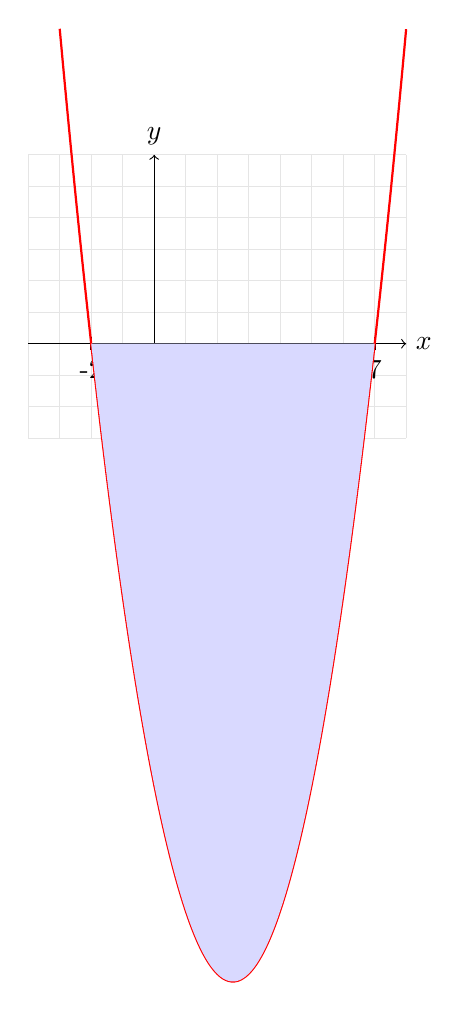
\begin{tikzpicture}[scale=0.4]
            % Light gray grid
            \draw[help lines, color=gray!20] (-4,-3) grid (8,6);
            
            % Axes
            \draw[->] (-4,0) -- (8,0) node[right] {$x$};
            \draw[->] (0,-3) -- (0,6) node[above] {$y$};
            
            % Root points and labels
            \foreach \x/\label in {-2/-2,7/7} {
                \draw[thick] (\x,0.2) -- (\x,-0.2) node[below] {\label};
            }
            
            % Parabola
            \draw[red,thick] plot[smooth,samples=100,domain=-3:8] (\x,{(\x)^2-5*\x-14});
            
            % Shaded region (solution)
            \fill[blue!15] (-2,0) -- plot[smooth,samples=100,domain=-2:7] (\x,{(\x)^2-5*\x-14}) -- (7,0) -- cycle;
        \end{tikzpicture}
    \end{columns}

    % Footer
    \begin{beamercolorbox}[wd=\paperwidth,ht=0.5cm,dp=0.2cm]{structure}
        \tiny
        \hspace{0.5cm}Created by Yi-Chen Lin \hfill Pre-Calculus 11 \hfill June 19, 2025 \hspace{0.5cm}
    \end{beamercolorbox}
\end{frame}

% Practice Problem 1
\begin{frame}{Practice Problem 1}
    \begin{tcolorbox}[colback=lightgray,colframe=accent,title=Practice 1]
        \footnotesize
        Solve the following square inequalities:
        \begin{enumerate}
            \item $x^2 > 25$
            \item $x^2 < 36$
            \item $x^2 \geq 49$
        \end{enumerate}
    \end{tcolorbox}
\end{frame}

\begin{frame}{Practice 1: Blank Number Lines}
    \begin{center}
    \begin{tikzpicture}[scale=0.7]
        % First number line
        \draw[->] (-8,-2) -- (8,-2);
        \foreach \x in {-5,0,5}
            \draw (\x,-1.8) -- (\x,-2.2) node[below] {\x};
        
        % Second number line
        \draw[->] (-8,0) -- (8,0);
        \foreach \x in {-6,0,6}
            \draw (\x,0.2) -- (\x,-0.2) node[below] {\x};
            
        % Third number line
        \draw[->] (-8,2) -- (8,2);
        \foreach \x in {-7,0,7}
            \draw (\x,2.2) -- (\x,1.8) node[below] {\x};
    \end{tikzpicture}
    \end{center}
\end{frame}

% Practice Problem 2
\begin{frame}{Practice Problem 2}
    \begin{tcolorbox}[colback=lightgray,colframe=accent,title=Practice 2]
        \footnotesize
        Solve the following quadratic inequalities:
        \begin{enumerate}
            \item $x^2 + 3x - 10 > 0$
            \item $2x^2 - 7x - 4 < 0$
        \end{enumerate}
    \end{tcolorbox}
\end{frame}

\begin{frame}{Practice 2: Blank Coordinate Planes}
    \begin{center}
    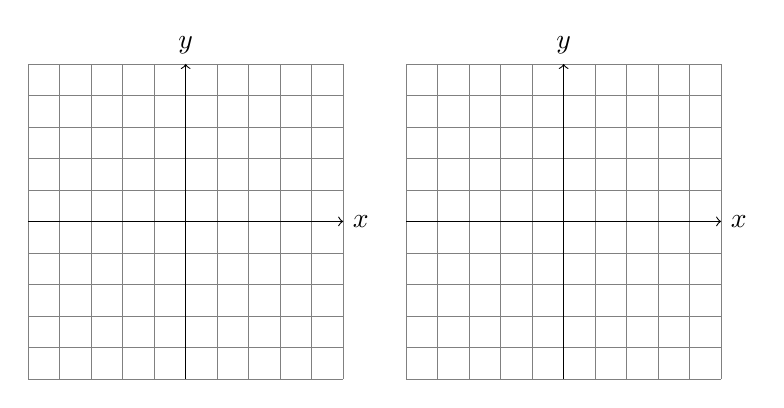
\begin{tikzpicture}[scale=0.4]
        % First coordinate plane
        \begin{scope}[xshift=-6cm]
            \draw[step=1cm,gray,very thin] (-5,-5) grid (5,5);
            \draw[->] (-5,0) -- (5,0) node[right] {$x$};
            \draw[->] (0,-5) -- (0,5) node[above] {$y$};
        \end{scope}
        
        % Second coordinate plane
        \begin{scope}[xshift=6cm]
            \draw[step=1cm,gray,very thin] (-5,-5) grid (5,5);
            \draw[->] (-5,0) -- (5,0) node[right] {$x$};
            \draw[->] (0,-5) -- (0,5) node[above] {$y$};
        \end{scope}
    \end{tikzpicture}
    \end{center}
\end{frame}

% Practice Problem 3
\begin{frame}{Practice Problem 3}
    \begin{tcolorbox}[colback=lightgray,colframe=accent,title=Practice 3]
        \footnotesize
        Write a quadratic inequality with the following solutions:
        \begin{enumerate}
            \item $-3 \leq x \leq 2$
            \item $x < -5$ or $x > 1$
        \end{enumerate}
    \end{tcolorbox}
\end{frame}

\begin{frame}{Practice 3: Blank Coordinate Planes}
    \begin{center}
    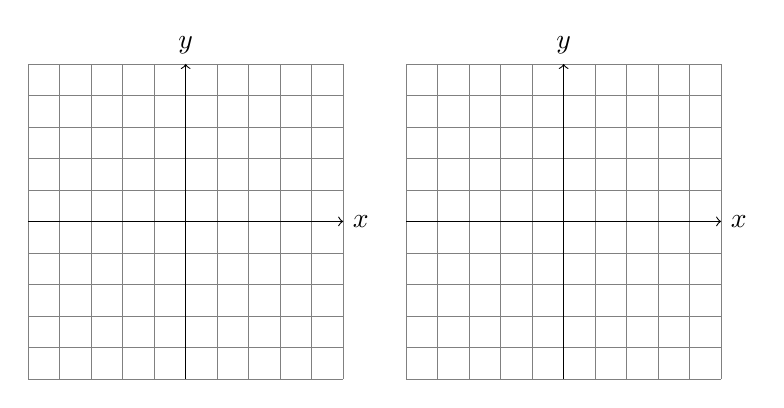
\begin{tikzpicture}[scale=0.4]
        % First coordinate plane
        \begin{scope}[xshift=-6cm]
            \draw[step=1cm,gray,very thin] (-5,-5) grid (5,5);
            \draw[->] (-5,0) -- (5,0) node[right] {$x$};
            \draw[->] (0,-5) -- (0,5) node[above] {$y$};
        \end{scope}
        
        % Second coordinate plane
        \begin{scope}[xshift=6cm]
            \draw[step=1cm,gray,very thin] (-5,-5) grid (5,5);
            \draw[->] (-5,0) -- (5,0) node[right] {$x$};
            \draw[->] (0,-5) -- (0,5) node[above] {$y$};
        \end{scope}
    \end{tikzpicture}
    \end{center}
\end{frame}

% Summary
\begin{frame}{Summary: Quadratic Inequalities}
    \begin{tcolorbox}[colback=lightgray,colframe=primary,title=Key Points]
        \footnotesize
        \begin{itemize}
            \item For \textcolor{accent}{square inequalities}:
            \begin{itemize}
                \item Take square root of both sides
                \item Consider both positive and negative solutions
            \end{itemize}
            \item For \textcolor{accent}{quadratic inequalities}:
            \begin{itemize}
                \item Factor first
                \item Find roots
                \item Test regions between and outside roots
            \end{itemize}
            \item Remember to:
            \begin{itemize}
                \item Always check your answer with test points
                \item Pay attention to inequality signs
                \item Consider the direction of the parabola
            \end{itemize}
        \end{itemize}
    \end{tcolorbox}
\end{frame}

\end{document} 